% ═══════════════════════════════════════════════════════════════════
% Unified B+A Manuscript for Classical and Quantum Gravity (CQG)
% Author: Gang Zhang
% Date: 2026-03-16
% ═══════════════════════════════════════════════════════════════════
\documentclass[12pt,a4paper]{article}

% ── Packages ────────────────────────────────────────────────────────
\usepackage[utf8]{inputenc}
\usepackage[T1]{fontenc}
\usepackage{lmodern}
\usepackage{amsmath,amssymb,amsfonts}
\usepackage{graphicx}
\usepackage{booktabs}
\usepackage{hyperref}
\usepackage[margin=2.5cm]{geometry}
\usepackage{enumitem}
\usepackage{caption}
\usepackage{float}
\usepackage{xcolor}
\usepackage{setspace}
\usepackage[numbers,sort&compress]{natbib}
\bibliographystyle{unsrtnat}

\hypersetup{
    colorlinks=true,
    linkcolor=blue!70!black,
    citecolor=blue!70!black,
    urlcolor=blue!70!black,
    hypertexnames=false,
}

% Graphics paths for figures from both B and A manuscripts
\graphicspath{{../manuscript_figures/}{../preA/manuscript_figures/}}

% Submission mode switch:
% \doubleblindtrue  -> anonymized manuscript for double-anonymous review
% \doubleblindfalse -> identified manuscript for single-anonymous review
\newif\ifdoubleblind
\doubleblindfalse

% ── Title ───────────────────────────────────────────────────────────
\title{Geometric Phase Transitions and Emergent Dimensional Selection\\
in Finite Causal Poset Ensembles}

\ifdoubleblind
\author{}
\date{}
\else
\author{Gang Zhang\thanks{Email: unicome@gmail.com}\\
\small Independent researcher}
\date{}
\fi

% ════════════════════════════════════════════════════════════════════
\begin{document}
\setstretch{1.2}
\maketitle

% ── Abstract ────────────────────────────────────────────────────────
\begin{abstract}
The Kleitman--Rothschild theorem implies that generic large finite posets are
three-layered and maximally entropic, creating an entropy catastrophe for any
program in which geometric causal order is expected to emerge dynamically. We
study whether this obstruction can be overcome in finite causal-poset ensembles
by a structurally motivated action that combines exact combinatorial entropy
with geometric penalty terms.

For Lorentzian-like 2D versus Kleitman--Rothschild competition, exact linear
extension counts on $N=10$--$44$ show that the transition threshold
$\gamma_c$ remains $O(1)$ across the full confirmatory range. Geometric
ablation reduces the effective backbone of the action to two indispensable
ingredients: global layer-shape balance ($g_{\mathrm{wh}}$) and a dimension
term. Replacing the original target-anchored dimension penalty by a
non-target-anchored consistency penalty $g_{\mathrm{con}}$ preserves the same
phase-transition structure while weakening the charge of circular
dimension-fixing.

We then test whether an action that rewards dimensional consistency, rather
than proximity to a preset target dimension, selects among Lorentzian
candidates. Across $N=20$--$72$, 4D Lorentzian-like posets dominate 92 of 98
scanned grid points under the consistency action, with positive pairwise
margins against both 2D and 3D competitors that increase with system size. This
pattern remains stable under seed variation and moderate weight perturbations.

These results are consistent with a two-step picture: finite-size geometric
phase emergence can occur without imposing continuum geometry directly, and
dimensional preference can arise from non-target-anchored structural
consistency constraints rather than from explicit dimension-specific priors.
\end{abstract}

\noindent\textbf{Keywords:} causal sets $\cdot$ posets $\cdot$ phase transition\\
\phantom{\noindent\textbf{Keywords:} }linear extensions $\cdot$
Kleitman--Rothschild $\cdot$ dimensional selection\\
\phantom{\noindent\textbf{Keywords:} }discrete quantum gravity

% ════════════════════════════════════════════════════════════════════
\section{Introduction}
\label{sec:intro}

The hypothesis that spacetime is fundamentally discrete---a locally finite
partial order (poset) whose elements are causally related events---lies at the
heart of causal set theory (CST)~\cite{bombelli1987,sorkin2005}. A central
challenge is the \emph{entropy catastrophe}: the Kleitman--Rothschild (KR)
theorem~\cite{kleitman1975} establishes that, asymptotically, almost all labeled
finite posets consist of three layers with bipartite random connectivity and
maximal linear extension count. If posets are weighted by the pure combinatorial
entropy $H = \log|L(P)|$, the partition function is overwhelmingly dominated by
these non-geometric, KR-type structures. How, then, can geometric order emerge?

Several strategies have been proposed. The Benincasa--Dowker (BD)
action~\cite{benincasa2010,benincasa2011} provides a discrete analogue of the
Einstein--Hilbert action on causal sets with a well-defined continuum limit.
In 2D, numerical work has found evidence for phase-transition-like behavior and
finite-size scaling in BD-based causal set quantum gravity
models~\cite{surya2012,glaser2018}, with related developments in dimensionally
restricted settings~\cite{cunningham2020}. Separately, Loomis and
Carlip~\cite{loomis2018} gave an analytic argument for suppression of a large
class of non-manifold-like causal sets (notably two-level orders) in a
Lorentzian path integral with Einstein--Hilbert weighting. Carlip~\cite{carlip2017}
and Surya~\cite{surya2019} provide broad reviews of dimensional reduction and
causal set quantum gravity, including discussions of causal set path sums and
their entropy challenges (see also Henson~\cite{henson2006} and
Dowker~\cite{dowker2005}). At a more combinatorial level, phase transitions in
random partial orders have been studied since Dhar~\cite{dhar1978} and
Pr{\"o}mel--Steger--Taraz~\cite{promel2001}. Despite this substantial body of
work, explicit finite-$N$ KR-versus-geometric competition curves computed with
exact linear-extension entropy remain scarce; here we provide a direct
$\gamma_c(N)$ scan with exact entropy in the confirmatory window $N=10$--$44$.

This paper addresses two open questions:

\begin{enumerate}[nosep]
\item \textbf{Bounded phase transition.} Does there exist a critical coupling
$\gamma_c$ at which geometric structures overtake KR-type posets, and does this
threshold remain bounded as $N$ grows?
\item \textbf{Dimensional selection.} If the action rewards dimensional
\emph{consistency} rather than proximity to a specific dimension, which
dimensionality does the dynamics prefer?
\end{enumerate}

Our approach proceeds through a ``diagnose $\to$ ablate $\to$ replace $\to$
predict $\to$ confirm'' sequence:

\begin{enumerate}[nosep]
\item We construct an 8-family ensemble with exact entropy ($N = 10$--$44$) and
find that $\gamma_c$ remains $O(1)$ across the confirmatory range
(Section~\ref{sec:bounded}).
\item Systematic ablation identifies a minimal backbone of two constraints
(Section~\ref{sec:ablation}).
\item Non-circular replacement of the target-anchored dimension term preserves
the phase transition (Section~\ref{sec:replacement}).
\item The replacement raises a concrete prediction: consistency constraints
should select higher-dimensional structures. We test this by extending the
ensemble to 4D and scanning $N = 20$--$72$
(Section~\ref{sec:dimensional}).
\item Robustness is confirmed through seed sensitivity, weight perturbation, and
out-of-grid validation (Section~\ref{sec:robustness}).
\end{enumerate}

% ════════════════════════════════════════════════════════════════════
\section{Framework}
\label{sec:framework}

\subsection{Poset ensemble}
\label{sec:ensemble}

We consider finite posets $P = (V, \leq)$ with $|V| = N$ elements, generating
samples from eight structurally distinct families organized in two tiers:

\medskip
\noindent\textbf{Tier-1 (geometric causal competition pool):}
\begin{itemize}[nosep]
\item \textbf{Lorentzian-like 2D} (\texttt{lor2d}): Sprinkling in $[0,1]^2$
with Minkowski lightcone order.
\item \textbf{Lorentzian-like 3D} (\texttt{lor3d}): Sprinkling in $[0,1]^3$
with lightcone order.
\item \textbf{Lorentzian-like 4D} (\texttt{lor4d}): Sprinkling in $[0,1]^4$
with lightcone order.
\item \textbf{KR-like} (\texttt{kr}): Three-layer bipartite posets with random
inter-layer edges, approximating the KR structure~\cite{kleitman1975}.
\item \textbf{Transitive percolation} (\texttt{tp}): Bernoulli percolation on a
linear order followed by transitive closure.
\end{itemize}

\noindent\textbf{Tier-2 (null-model stress tests):}
\begin{itemize}[nosep]
\item \textbf{Multi-layer random} (\texttt{mlr}): 4 equal layers with random
$p = 0.5$ inter-layer edges.
\item \textbf{Interval order} (\texttt{int}).
\item \textbf{Absolute layered} (\texttt{abs}).
\end{itemize}

These Tier-2 families are chosen as ``nearby'' high-entropy competitors in the
space of finite posets: beyond KR-type three-layer orders, enumerative results
show that other layered structures (two-layer, four-layer, etc.) are likewise
abundant and can dominate naive counting measures~\cite{promel2001}. We include
representatives of these classes to probe the discriminative limits of any
candidate action.

All Lorentzian-like families are constructed via causal set
sprinkling~\cite{bombelli1987}: $N$ points are sprinkled uniformly in $[0,1]^d$
with coordinates $(t, x_1, \ldots, x_{d-1})$. The causal relation is
\begin{equation}
    i \prec j \iff \Delta t_{ij} > 0 \;\text{ and }\;
    (\Delta t_{ij})^2 \geq \sum_{k=1}^{d-1} (\Delta x_k)^2,
    \label{eq:causal}
\end{equation}
where $\Delta t_{ij} = t_j - t_i$, followed by transitive closure.

For the bounded phase-transition analysis
(Sections~\ref{sec:bounded}--\ref{sec:replacement}), we use the original
7-family ensemble: \texttt{lor2d}, \texttt{lor3d}, \texttt{kr},
\texttt{mlr}, \texttt{tp}, \texttt{int}, and \texttt{abs}. The confirmatory
exact scan covers $N \in \{10, 12, 14, 16, 20, 24, 28, 32, 36, 40, 44\}$ with
$K = 5$ samples per family per $N$. For the dimensional selection analysis
(Section~\ref{sec:dimensional}), we use the 4-family subset (\texttt{lor2d},
\texttt{lor3d}, \texttt{lor4d}, \texttt{kr}) with
$N \in \{20, 24, 28, \ldots, 72\}$ ($14$ sizes) and $K = 8$ samples for
$N \leq 40$, $K = 4$ for $N > 40$.

The tier distinction separates families by generative mechanism:
Tier-1 families are generated by embedding points in a metric spacetime (or a
combinatorial standard model), while Tier-2 families are purely combinatorial
layered constructions. The Prediction~B core claim ($\gamma_c$ boundedness) is
evaluated exclusively within Tier-1. Tier-2 families serve as stress tests that
define the \emph{discriminative ceiling} of the current action
(Section~\ref{sec:discussion}).

\subsection{Exact linear extension count}
\label{sec:exact}

We define $H(P) = \log |L(P)|$ where $L(P)$ is the set of linear extensions,
computed exactly via dynamic programming over
antichains~\cite{brightwell1991}. The cost depends strongly on antichain
structure: sub-second for \texttt{lor2d} at $N = 48$, about $3.8$\,s at
$N = 72$, about $33.8$\,s at $N = 88$, and about $127.4$\,s at $N = 104$, but
already $56$\,s for \texttt{kr} at $N = 44$. For \texttt{lor3d}, exact
evaluation reaches $N = 56$ ($327$\,s). This asymmetry motivates the
one-sided exact extension strategy adopted for large-$N$ probes
(Figure~\ref{fig:timing}).

The use of $\log|L(P)|$ is not meant as a thermodynamic entropy of matter
fields, but as a \emph{combinatorial measure term}: for an unlabeled poset $P$,
the number of natural labelings consistent with the order is precisely the
number of linear extensions, so a labeled path sum (or any proxy that samples
labelings rather than isomorphism classes) implicitly weights $P$ by
$|L(P)|$. Such entropy factors and their competition with action terms in
causal set path sums have been discussed in the CST literature; see for example
Mathur, Singh, and Surya~\cite{mathur2021}.

This is a choice of ensemble and measure, not a claim that $\log|L(P)|$ is the
unique or physically correct definition of gravitational entropy. One may
instead formulate a path sum over \emph{unlabeled} posets, with a measure that
divides by automorphism factors (e.g.\ weights proportional to $1/|\mathrm{Aut}(P)|$)
or uses other gauge-fixing conventions. Such alternatives change the effective
entropy term and can modify which families dominate. Our goal here is more
modest: to analyze finite-$N$ competition in the labeled (or label-sampling)
setting in which linear extensions arise as the natural combinatorial measure
factor.

For the 4-family dimensional selection experiments at $N > 32$, linear extension
counts for \texttt{kr}, \texttt{lor3d}, and \texttt{lor4d} are estimated via
Sequential Importance Sampling (SIS, 4096 runs). As a cross-check, SIS versus
exact counts at $N = 20$--$36$ yield a mean absolute error of $0.074$ in
$\log|L(P)|$ ($\sim 2.3\%$), well below observed winning margins.

\subsection{Action definition}
\label{sec:action}

Three action paths separate neutral and geometric contributions:
\begin{align}
    A_1 &= -\beta H + \gamma \cdot I_{\text{neutral}}, \label{eq:A1} \\
    A_2 &= -\beta H + \gamma \cdot (I_{\text{neutral}} + I_{\text{geo}}),
    \label{eq:A2} \\
    A_3 &= -\beta H + \gamma \cdot I_{\text{geo}}, \label{eq:A3}
\end{align}
with $\beta = 1$. The geometric penalty decomposes into seven sub-terms:
width-height balance ($g_{\text{wh}}$), dimension proxy ($g_{\text{dim}}$),
interval shape ($g_{\text{int}}$), comparability window ($g_{\text{cmp}}$),
cover density ($g_{\text{cov}}$), interval profile ($g_{\text{prf}}$), and
layer smoothness ($g_{\text{lyr}}$), each normalized to $[0,1]$.

The critical coupling is:
\begin{equation}
    \gamma_c(N) = \inf\bigl\{\gamma > 0 :
    \bar{S}_{\texttt{lor2d}}(\gamma) < \bar{S}_{\texttt{kr}}(\gamma)\bigr\}.
    \label{eq:gamma_c}
\end{equation}

For the dimensional selection experiments, we additionally define two
replacement actions:
\begin{itemize}[nosep]
\item \textbf{$A_2$ consistency}: Replace $g_{\text{dim}}$ with
$g_{\text{con}}$ (Eq.~\ref{eq:gcon}).
\item \textbf{$A_2$ multi-consistency}: Replace $g_{\text{dim}}$ with
$g_{\text{mcon}}$ (Eq.~\ref{eq:gmcon}).
\end{itemize}

% ════════════════════════════════════════════════════════════════════
\section{Bounded Phase Transition}
\label{sec:bounded}

Under $A_2$, $\gamma_c$ exists for all tested $N$ and remains $O(1)$:

\begin{table}[h]
\centering
\caption{Critical coupling $\gamma_c$ under $A_2$ (exact entropy). All values
for $N \geq 12$ lie in $[0.146, 0.995]$.}
\label{tab:gamma_c}
\begin{tabular}{@{}lcccccc@{}}
\toprule
$N$ & 10 & 12 & 14 & 16 & 20 & 24 \\
\midrule
$\gamma_c$ & 9.19 & 0.744 & 0.781 & 0.693 & 0.146 & 0.262 \\
\bottomrule
\end{tabular}
\medskip

\begin{tabular}{@{}lcccccc@{}}
\toprule
$N$ & 28 & 32 & 36 & 40 & 44 & \\
\midrule
$\gamma_c$ & 0.995 & 0.694 & 0.570 & 0.248 & 0.149 & \\
\bottomrule
\end{tabular}
\end{table}

For $N \geq 12$, all $\gamma_c$ values lie in $[0.146, 0.995]$
(Figure~\ref{fig:gamma_c}). Under $A_1$ (neutral terms only), no crossing
exists at any tested~$N$, confirming that geometric penalties are necessary.

\begin{figure}[h]
    \centering
    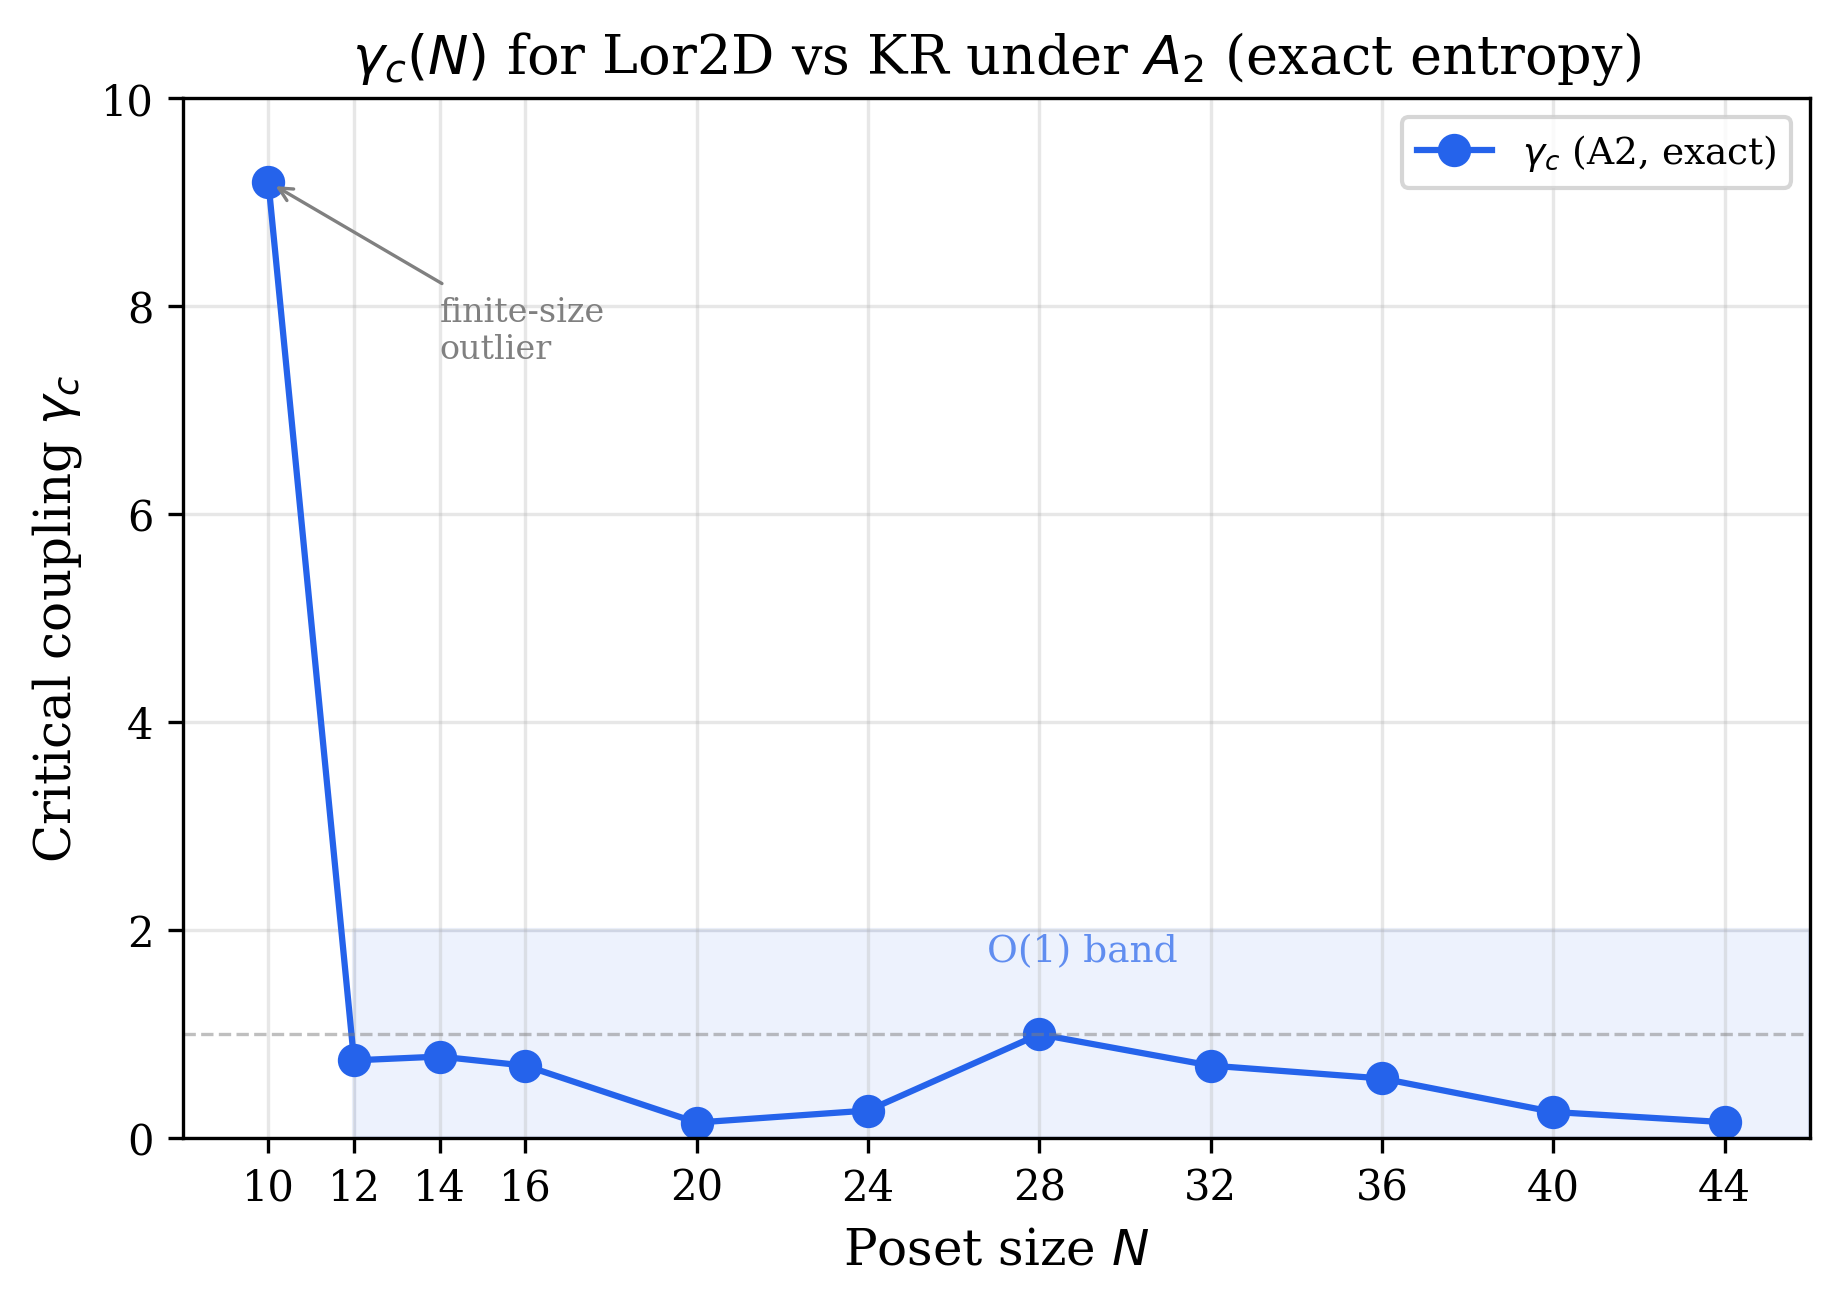
\includegraphics[width=\columnwidth]{fig1_gamma_c_curve.png}
    \caption{$\gamma_c(N)$ under $A_2$. Inset: $N \geq 12$ detail showing
    all values in $[0.15, 1.00]$.}
    \label{fig:gamma_c}
\end{figure}

\subsection{Exact-timing frontier}
\label{sec:timing}

One-sided exact evaluation for \texttt{lor2d} remains feasible up to $N = 104$,
while \texttt{kr} becomes computationally intractable beyond $N \approx 44$.
For \texttt{lor3d}, exact evaluation extends to $N = 56$ ($280$\,s at $N = 48$,
$288$\,s at $N = 52$, $327$\,s at $N = 56$). This asymmetry supports an
asymmetric exact-plus-mixed extension strategy beyond the confirmatory window
(Figure~\ref{fig:timing}).

\begin{figure}[h]
    \centering
    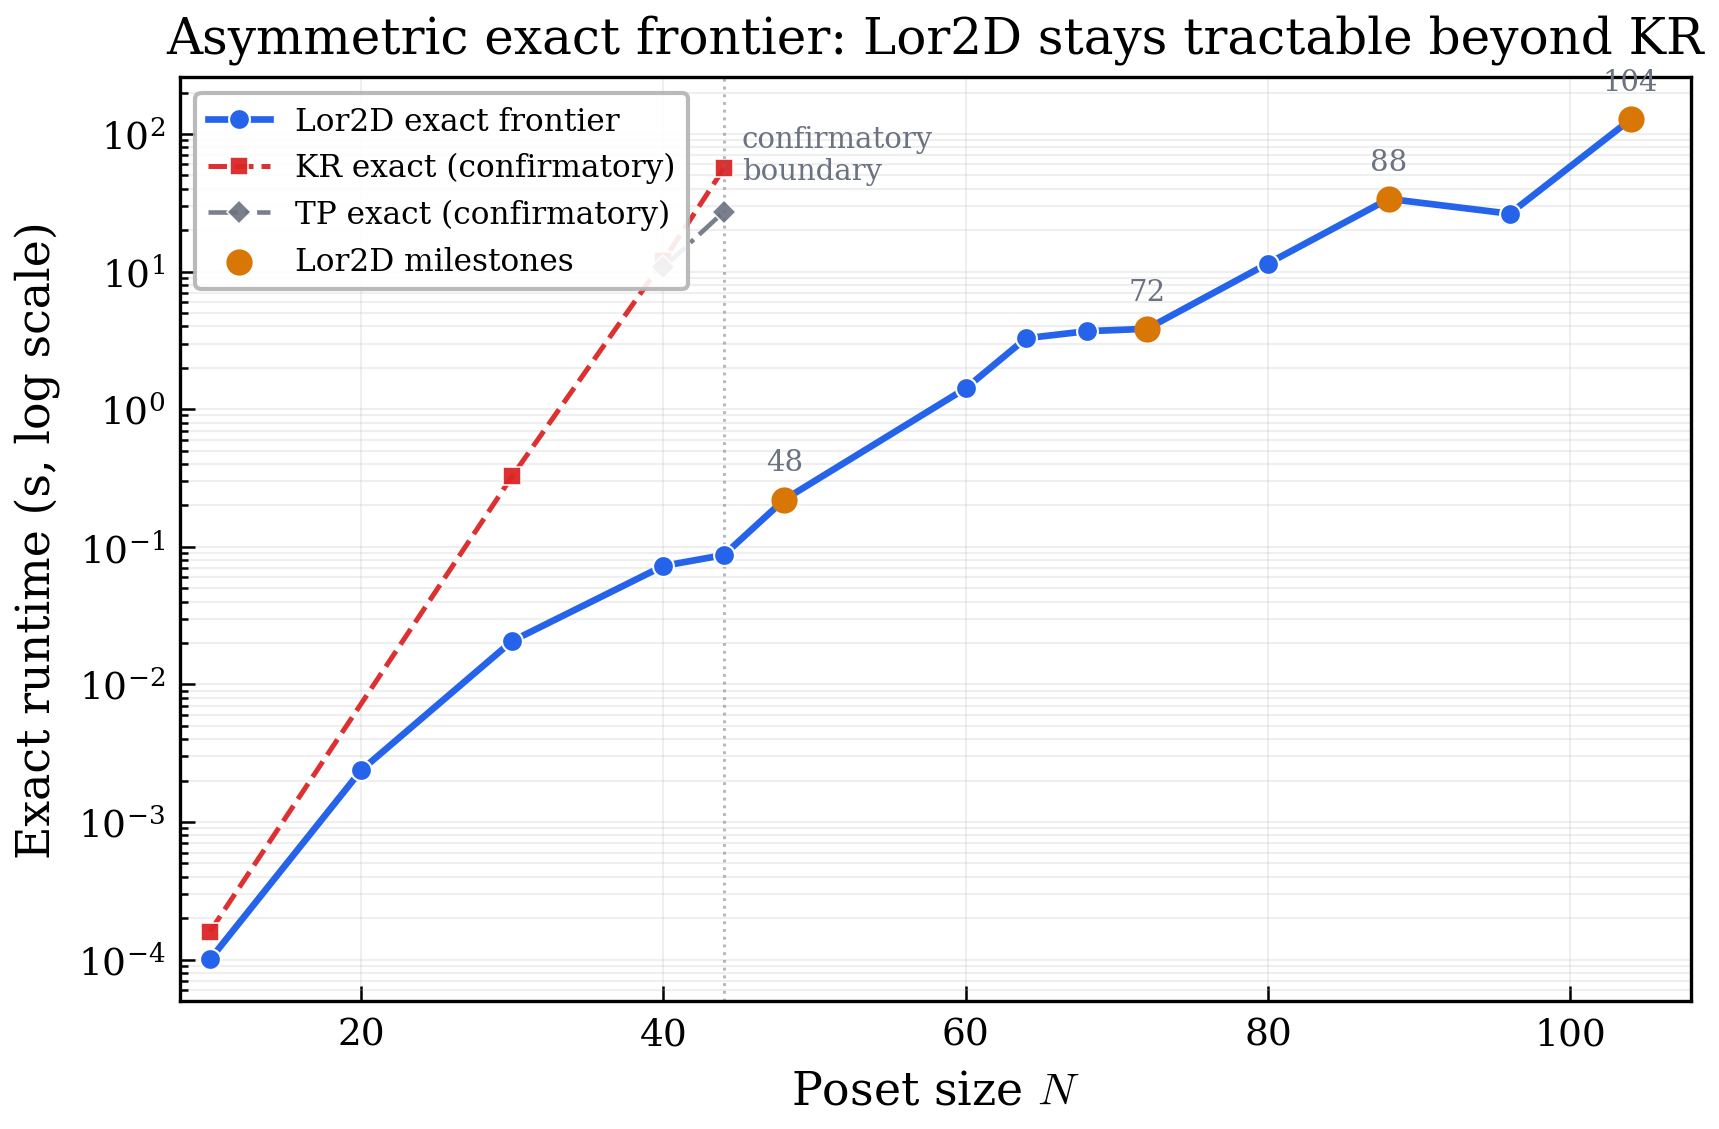
\includegraphics[width=\columnwidth]{fig4_exact_timing_frontier.png}
    \caption{Exact-timing frontier. Single-sided exact evaluation remains
    practical for \texttt{lor2d} up to $N = 104$, while \texttt{kr} and other
    families become expensive much earlier.}
    \label{fig:timing}
\end{figure}

\subsection{Near-wall mixed extension}
\label{sec:nearwall}

Beyond $N = 44$, we use an asymmetric mixed protocol: exact entropy for
\texttt{lor2d} and SIS-based estimation for \texttt{kr}. At $N = 52$ and $56$,
the $A_2^{\mathrm{full}}$ score curves show no crossing up to $\gamma = 2.0$,
but the gap contracts to near-degeneracy
($\Delta A_{\mathrm{KR\text{-}L2D}} \approx -0.20$ at $N = 52$ and
$\approx -0.84$ at $N = 56$), indicating that the competition remains
structurally active beyond the exact confirmatory range
(Figure~\ref{fig:nearwall}).

\begin{figure}[h]
    \centering
    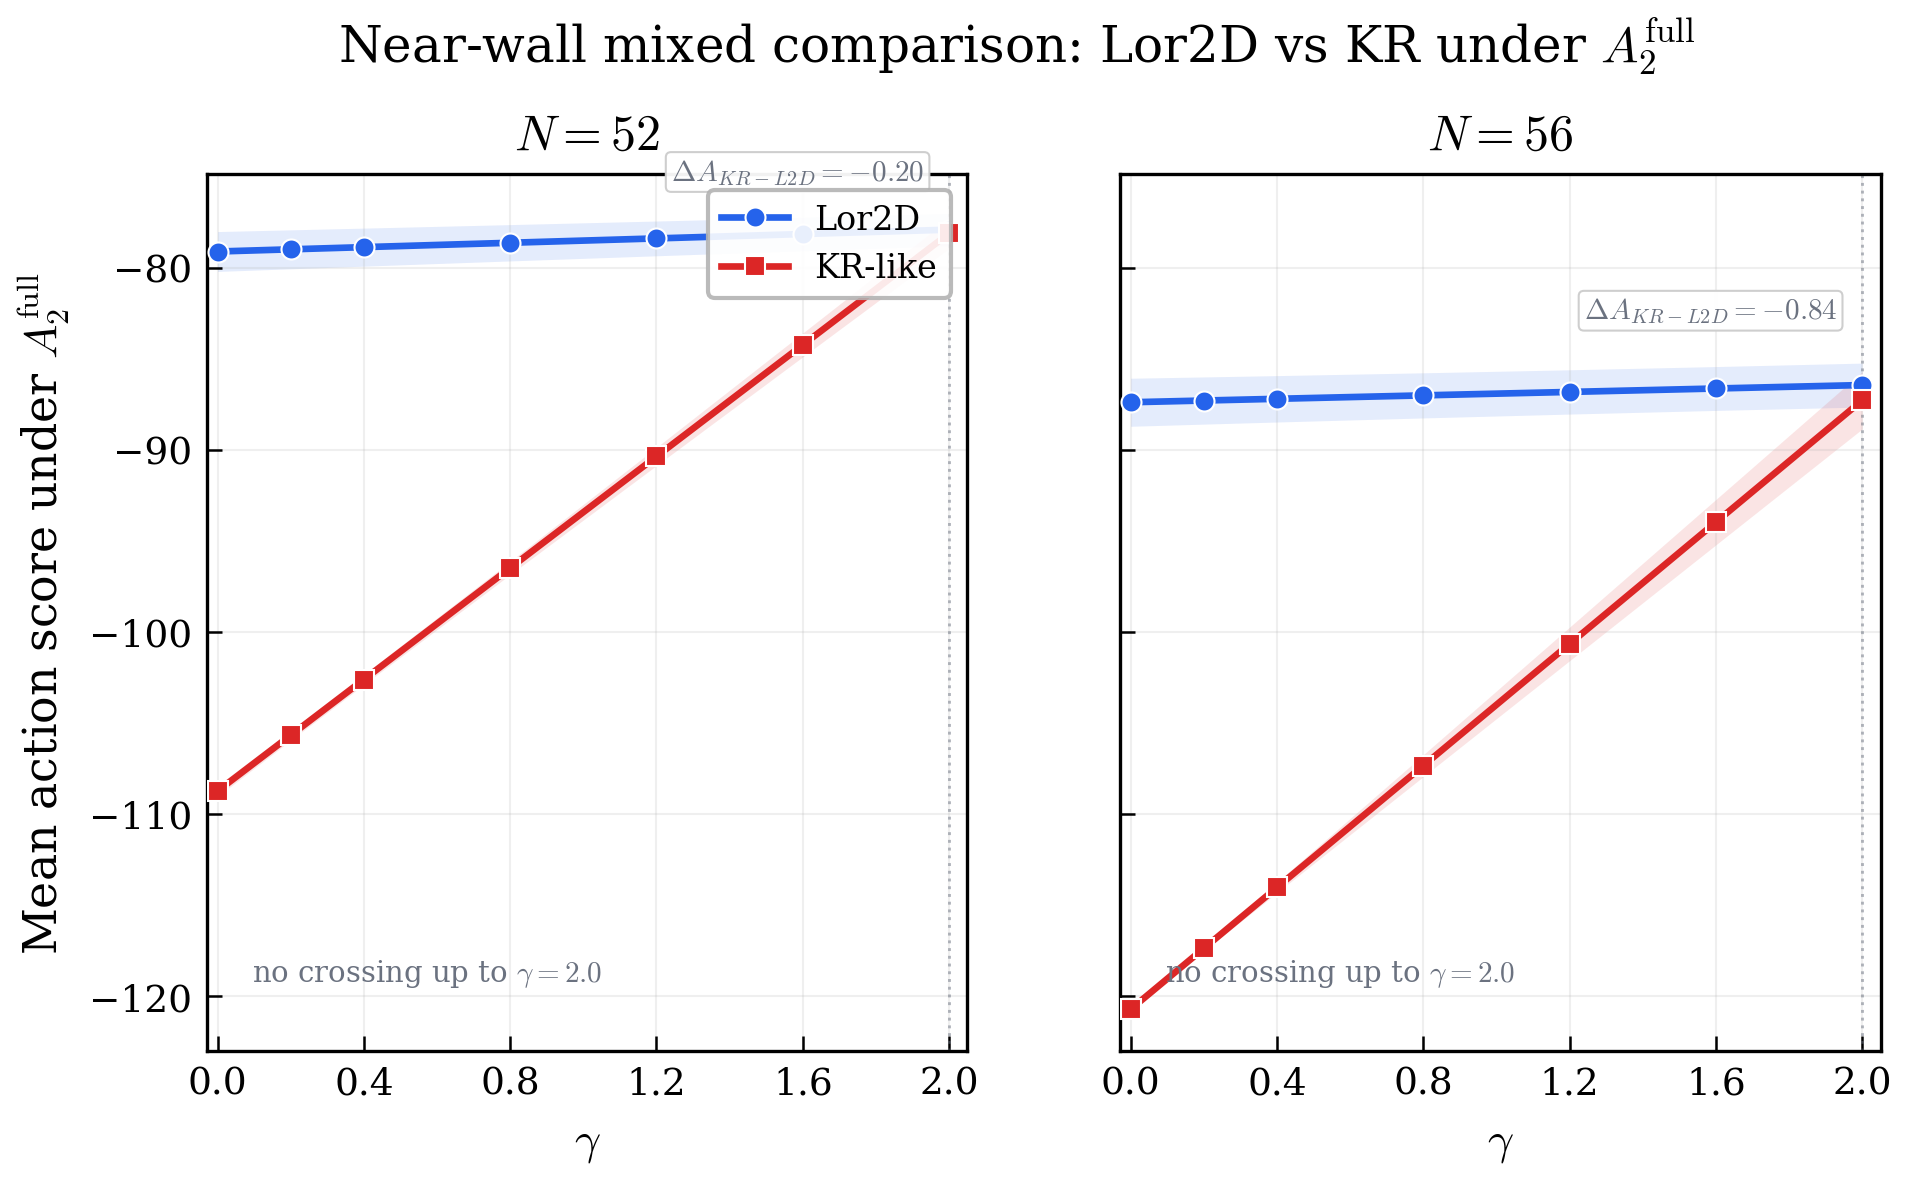
\includegraphics[width=\columnwidth]{fig5_mixed_lor2d_vs_kr.png}
    \caption{Near-wall mixed extension for $A_2^{\mathrm{full}}$ at $N = 52$
    and $56$. Solid lines: mean scores; shaded bands: one standard deviation.
    No crossing is observed up to $\gamma = 2.0$, but the gap contracts to
    near-degeneracy at the high-$\gamma$ boundary.}
    \label{fig:nearwall}
\end{figure}

% ════════════════════════════════════════════════════════════════════
\section{Ablation and Minimal Backbone}
\label{sec:ablation}

\subsection{Ablation of geometric sub-terms}
\label{sec:ablation_b}

Systematic single-term removal within the 7-family ensemble identifies two
critical sub-terms: $g_{\text{wh}}$ (fails from $N \geq 36$) and $g_{\text{dim}}$
(fails at $N = 36, 44$). Combined removal of both eliminates all crossings.
Removing non-critical terms has no effect. This establishes a
\emph{backbone--shell} structure: $g_{\text{wh}}$ and $g_{\text{dim}}$ form the
minimal backbone, while the remaining five terms constitute an outer shell
(Figure~\ref{fig:ablation}).

\begin{figure}[h]
    \centering
    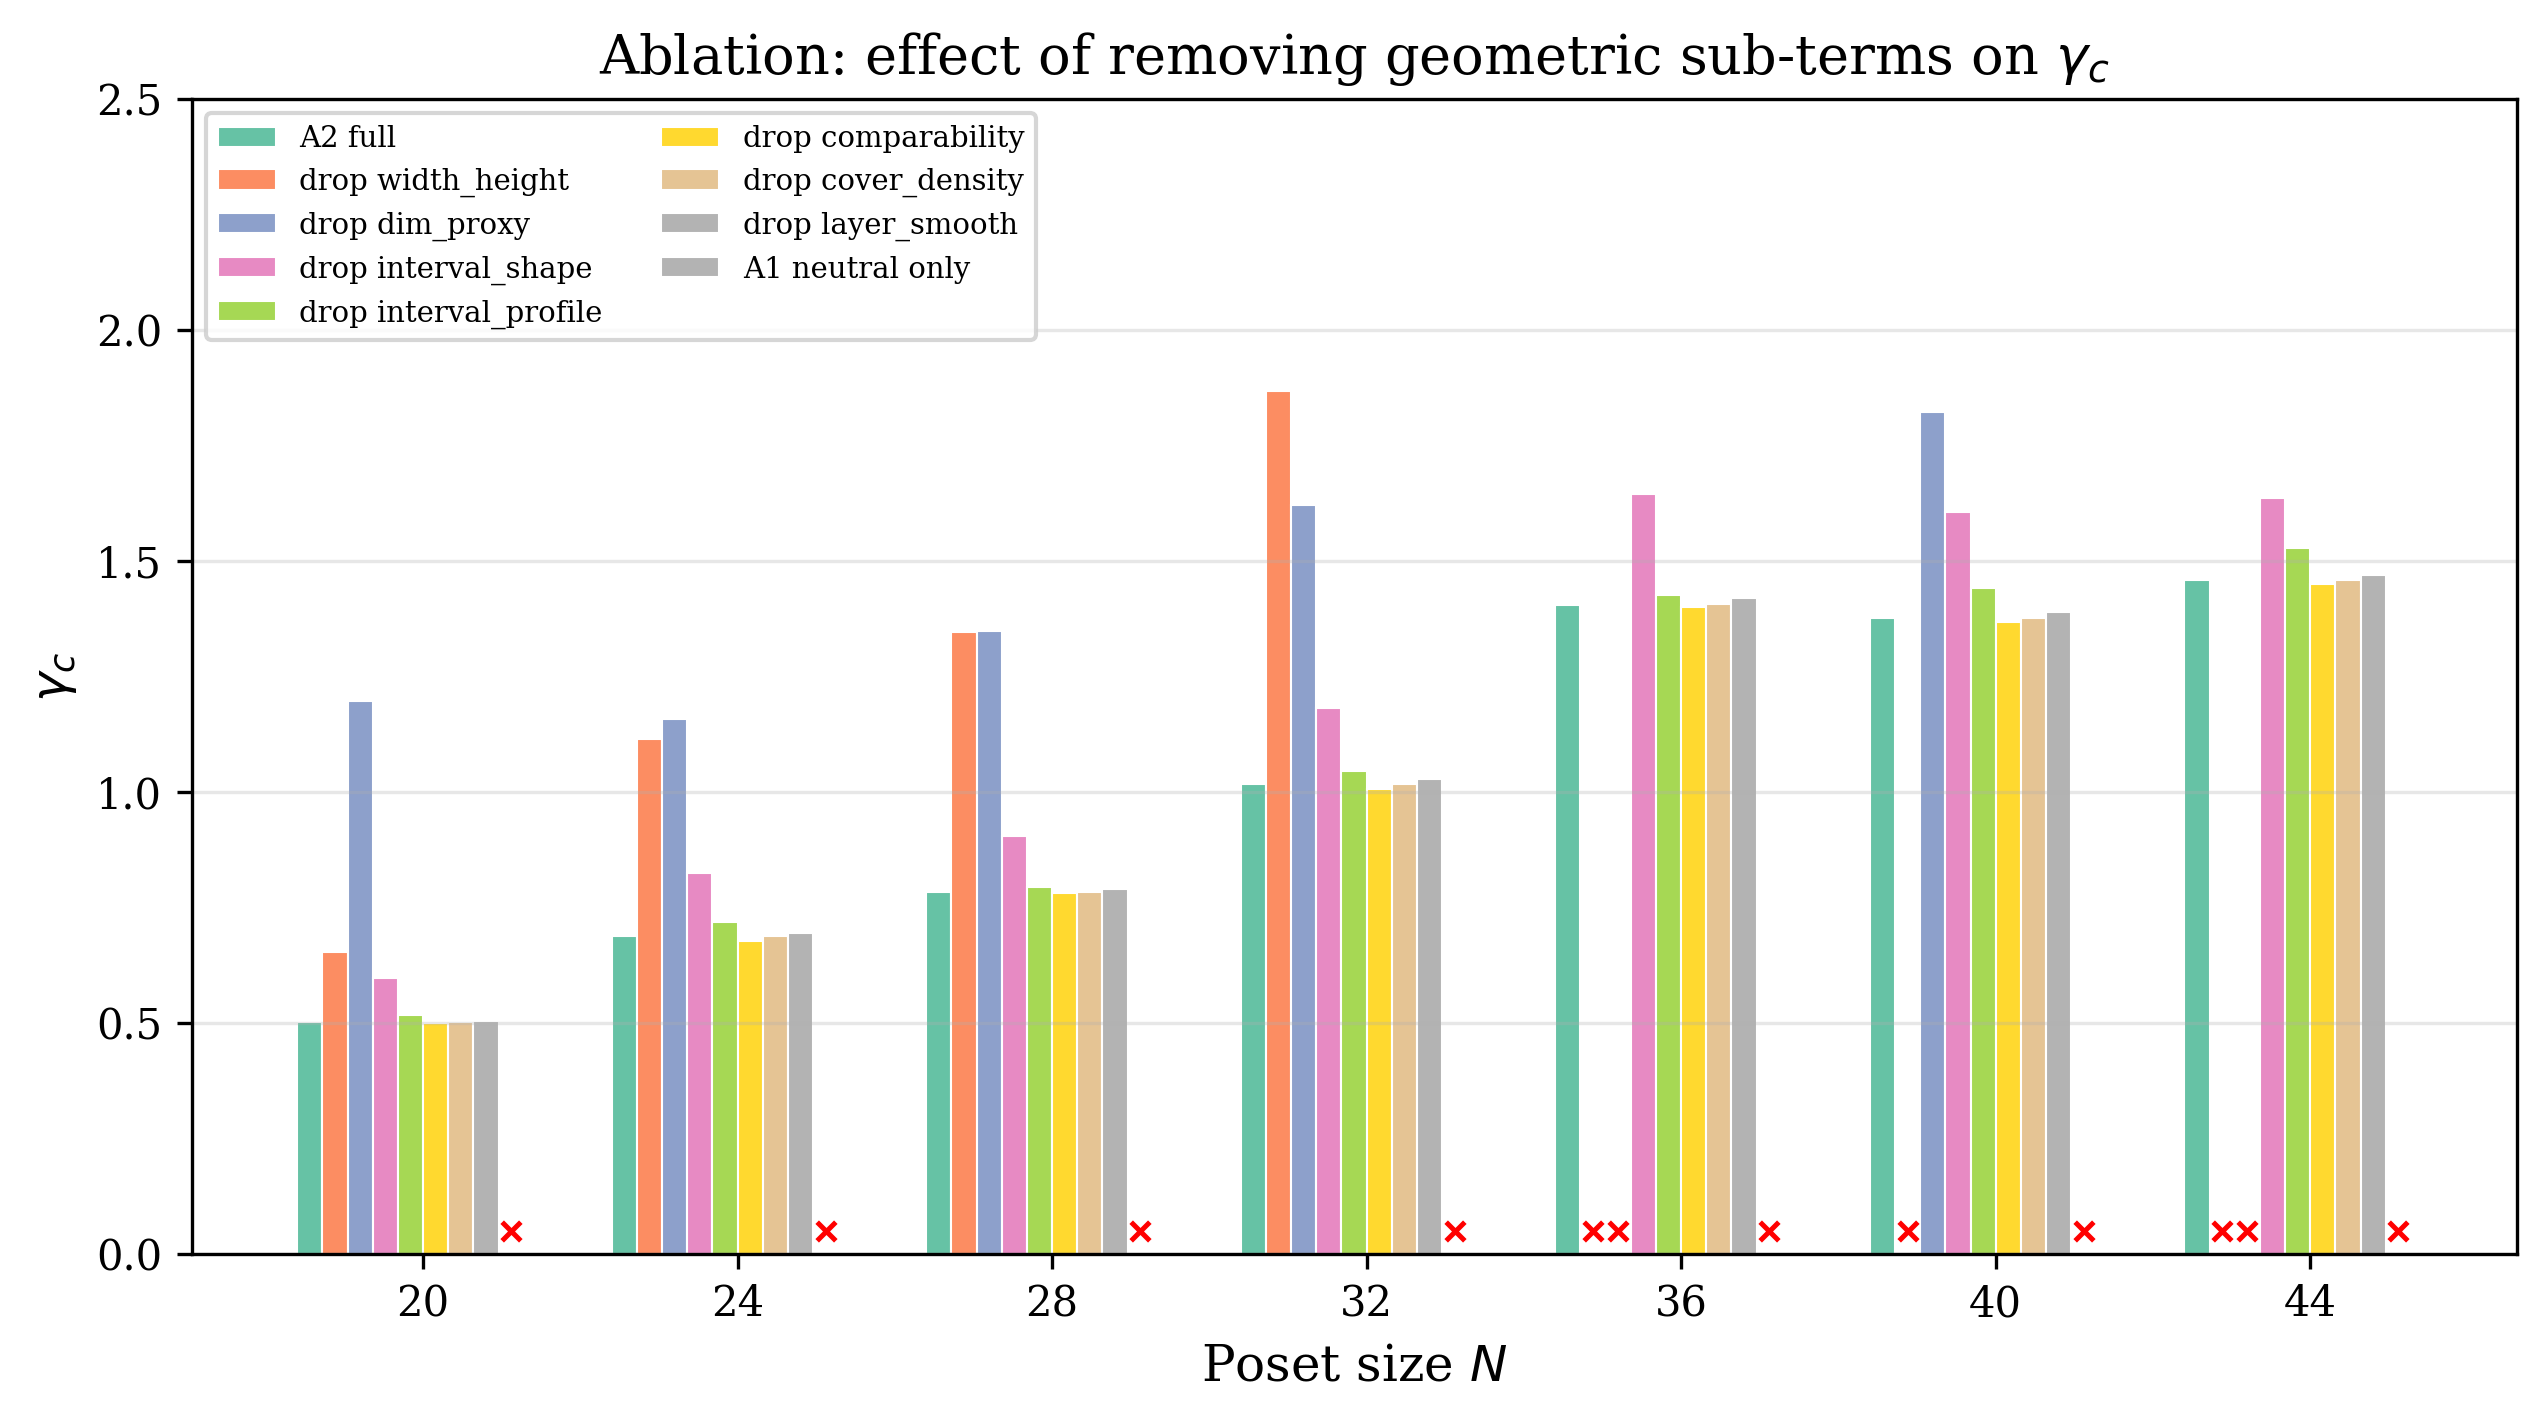
\includegraphics[width=\columnwidth]{fig2_ablation_summary.png}
    \caption{Ablation heatmap: $\gamma_c$ per variant and $N$. Removing
    $g_{\text{wh}}$ or $g_{\text{dim}}$ alone destroys the phase transition
    at large $N$; the remaining five terms are non-critical.}
    \label{fig:ablation}
\end{figure}

\subsection{Ablation in the 4-family ensemble}
\label{sec:ablation_a}

The same ablation pattern appears in the 4-family dimensional selection ensemble.
Under the original $A_2$ full action, the 4D family does \emph{not} achieve
stable dominance; across 98 $(N, \gamma)$ configurations the winner counts are:
\texttt{lor4d}~36, KR~35, \texttt{lor2d}~19, \texttt{lor3d}~8. Removing
$g_{\text{dim}}$ alone causes \texttt{lor4d} wins to jump from 10 to 28 (out of
35 configurations at $N = 20$--$36$), while KR wins drop to~0. The dimension
term creates a ``glass ceiling'' that prevents \texttt{lor4d} from expressing its
structural advantages (Table~\ref{tab:ablation_a}).

\begin{table}[h]
\centering
\caption{Winner counts under systematic ablation in the 4-family ensemble
($N = 20$--$36$, 35 configurations each).}
\label{tab:ablation_a}
\begin{tabular}{lcccc}
\toprule
\textbf{Variant} & \textbf{Lor4D} & \textbf{KR} & \textbf{Lor2D} &
\textbf{Lor3D} \\
\midrule
$A_2$ full (baseline) & 10 & 9 & 14 & 2 \\
$A_2$ no-dim & 28 & 0 & 1 & 6 \\
$A_2$ no-wh & 10 & 22 & 3 & 0 \\
$A_2$ interval-only & 35 & 0 & 0 & 0 \\
\bottomrule
\end{tabular}
\end{table}

% ════════════════════════════════════════════════════════════════════
\section{Non-Circular Replacement}
\label{sec:replacement}

We replace the target-anchored $g_{\text{dim}}$ with a consistency penalty:
\begin{equation}
    g_{\text{con}}(P) = \mathrm{Var}[d_{\text{local}}]
    + (\overline{d}_{\text{local}} - d_{\text{global}})^2,
    \label{eq:gcon}
\end{equation}
where $d_{\text{local}}$ is the order-fraction dimension proxy applied to
sampled causal intervals with $|I| \geq 4$, and $d_{\text{global}}$ is the
same estimator applied to the full poset. This penalizes dimensional
\emph{inconsistency} without specifying a target dimension.

As a robustness check, we define a multi-estimator consistency penalty requiring
agreement across three independent coarse-grained dimension proxies:
\begin{equation}
    g_{\text{mcon}}(P) = \mathrm{Var}[d_{\text{order}}, d_{\text{chain}},
    d_{\text{width}}]
    + \sum_{e \in \{\text{order, chain, width}\}} g_{\text{con}}^{(e)}(P).
    \label{eq:gmcon}
\end{equation}

\subsection{Phase-transition preservation}

The replacement preserves $\gamma_c$ at all $N = 20$--$44$ within the 7-family
ensemble (Figure~\ref{fig:replacement}). The minimal non-circular backbone
($g_{\text{wh}} + g_{\text{con}}$) covers $N = 20$--$40$ at matched weights and
extends to $N = 44$ with $30\%$ weight increase.

Extending the scan beyond the confirmatory exact window, the consistency backbone
continues to recover a crossing at $N = 48$ and $N = 52$ in exploratory
mixed-exact runs, yielding recovery factors $c_{44} \approx 1.41$,
$c_{48} \approx 1.69$, and $c_{52} \approx 1.80$ (seed-sensitive). The
sequence rises slowly and remains $O(1)$, showing no sign of accelerating
divergence.

\begin{figure}[h]
    \centering
    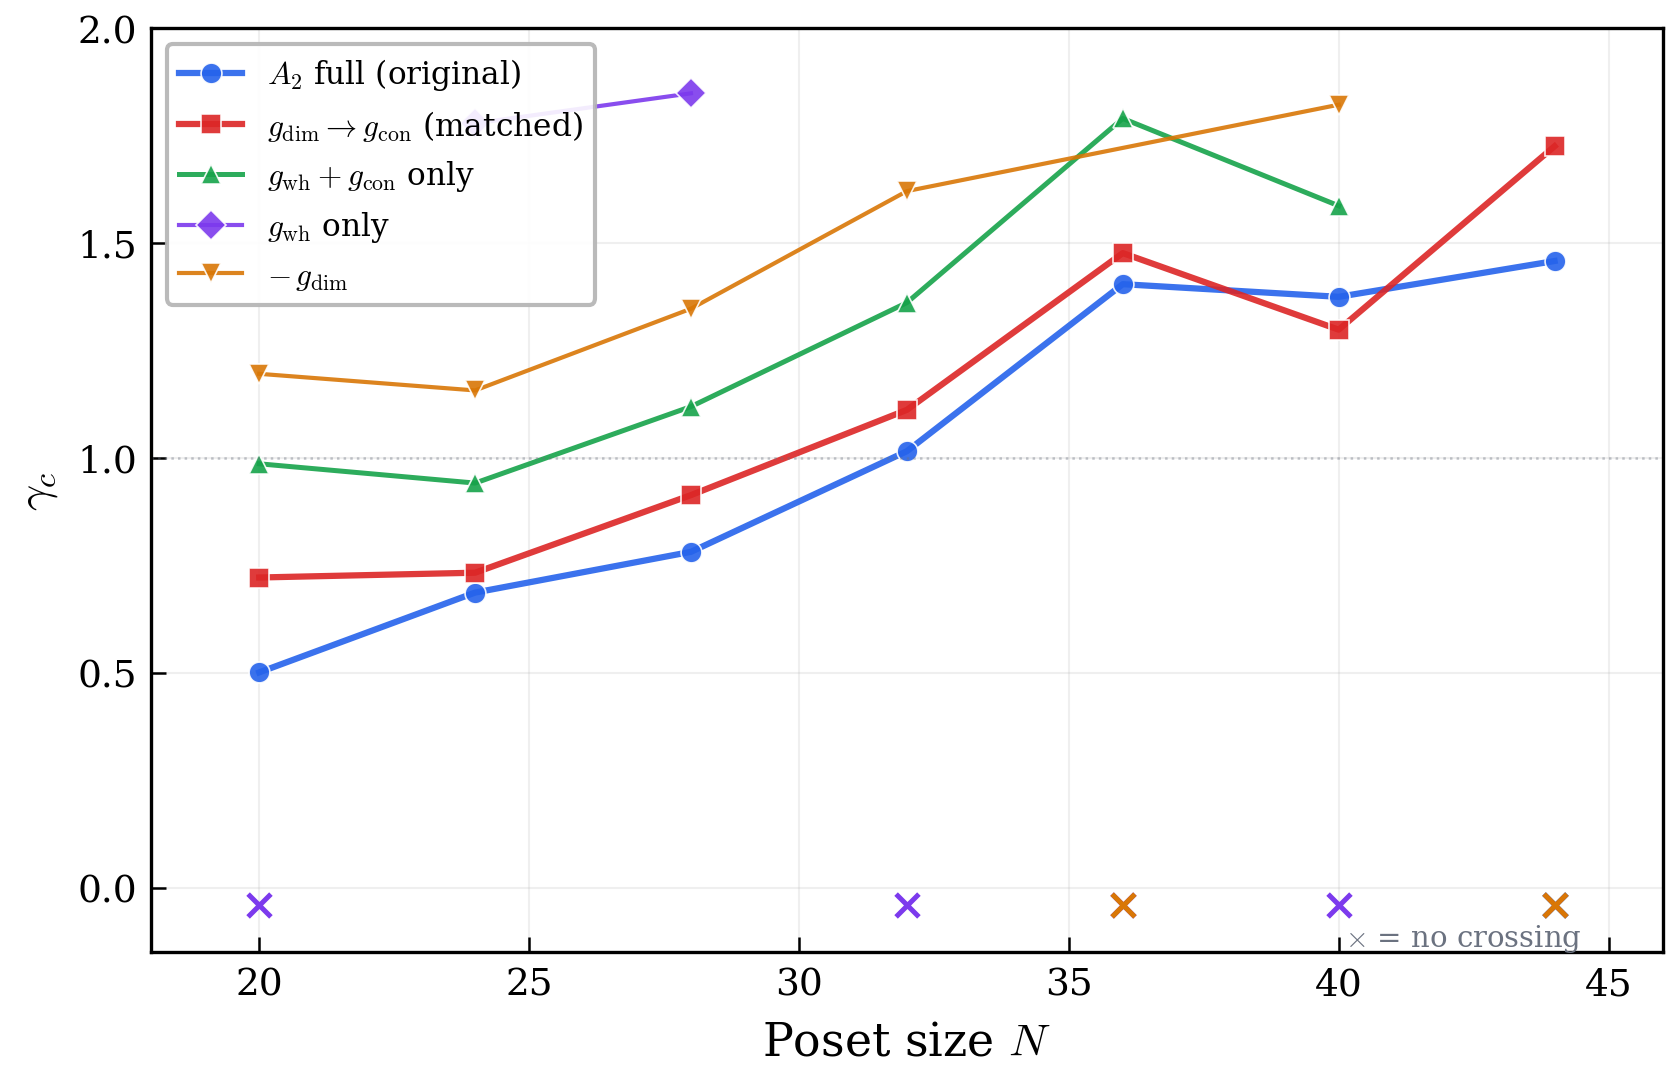
\includegraphics[width=\columnwidth]{fig3_noncircular_replacement.png}
    \caption{Non-circular replacement: $\gamma_c$ under different backbones.
    The consistency-based backbone preserves the bounded phase transition.}
    \label{fig:replacement}
\end{figure}

% ════════════════════════════════════════════════════════════════════
\section{Dimensional Selection}
\label{sec:dimensional}

The non-circular replacement raises a natural prediction: if the action rewards
dimensional \emph{consistency} rather than proximity to a specific~$d$, then
among Lorentzian-like structures of different dimensionality, which dimension
does the action prefer? The 4D family has (i)~higher entropy $H$ (the stricter
causal condition in more spatial dimensions yields a lower comparable fraction
and hence more linear extensions), (ii)~higher $g_{\text{dim}}$ penalty (since
$d_{\mathrm{eff}} \approx 4 \neq 2$), and (iii)~\emph{lower} $g_{\text{con}}$
penalty (strong internal dimensional coherence). The consistency replacement
should therefore unlock 4D dominance.

\subsection{Consistency replacement yields 4D dominance}
\label{sec:4d_dominance}

Under the consistency replacement, \texttt{lor4d} wins 92 out of 98
$(N, \gamma)$ configurations. Both KR and \texttt{lor2d} \emph{never} win. The
multi-estimator variant yields a nearly identical pattern ($89/98$), confirming
estimator independence (Table~\ref{tab:replacement}).

\begin{table}[h]
\centering
\caption{Winner counts: original vs.\ consistency replacement (98
configurations each, $N = 20$--$72$, $\gamma \in \{0, 0.2, \ldots, 2.0\}$).}
\label{tab:replacement}
\begin{tabular}{lcccc}
\toprule
\textbf{Variant} & \textbf{Lor4D} & \textbf{KR} & \textbf{Lor2D} &
\textbf{Lor3D} \\
\midrule
$A_2$ full (original) & 36 & 35 & 19 & 8 \\
$A_2$ consistency ($g_{\text{con}}$) & 92 & 0 & 0 & 6 \\
$A_2$ multi-con.\ ($g_{\text{mcon}}$) & 89 & 0 & 0 & 9 \\
\bottomrule
\end{tabular}
\end{table}

Against \texttt{lor2d} specifically, \texttt{lor4d} wins all 98 pairwise
comparisons ($100\%$). The 6 non-\texttt{lor4d} wins go to \texttt{lor3d} at
small-$N$, high-$\gamma$ configurations where geometric penalties dominate and
the entropy advantage of \texttt{lor4d} is insufficient to compensate.

\subsection{Growing margin of victory}
\label{sec:margin}

The margin of \texttt{lor4d} over both competitors shows a strong upward trend
with~$N$ under $A_2$ consistency (Table~\ref{tab:margin},
Figure~\ref{fig:margin}).

\begin{table}[h]
\centering
\caption{Mean margin of \texttt{lor4d} over competitors under $A_2$
consistency, averaged across $\gamma$.}
\label{tab:margin}
\begin{tabular}{ccccc}
\toprule
$N$ & vs Lor2D & vs Lor2D & vs Lor3D & vs Lor3D \\
    & (mean)   & (min)    & (mean)   & (min) \\
\midrule
20 & 7.41 & 1.70 & 2.27 & $-0.17$ \\
28 & 14.21 & 7.77 & 2.59 & $-2.07$ \\
36 & 19.30 & 11.41 & 4.20 & $-1.72$ \\
44 & 27.12 & 19.42 & 6.02 & 0.36 \\
52 & 36.22 & 30.40 & 11.29 & 7.27 \\
60 & 45.41 & 38.88 & 14.50 & 10.02 \\
68 & 50.82 & 41.51 & 16.41 & 9.44 \\
72 & 56.72 & 47.15 & 16.53 & 10.06 \\
\bottomrule
\end{tabular}
\end{table}

\begin{figure}[h]
    \centering
    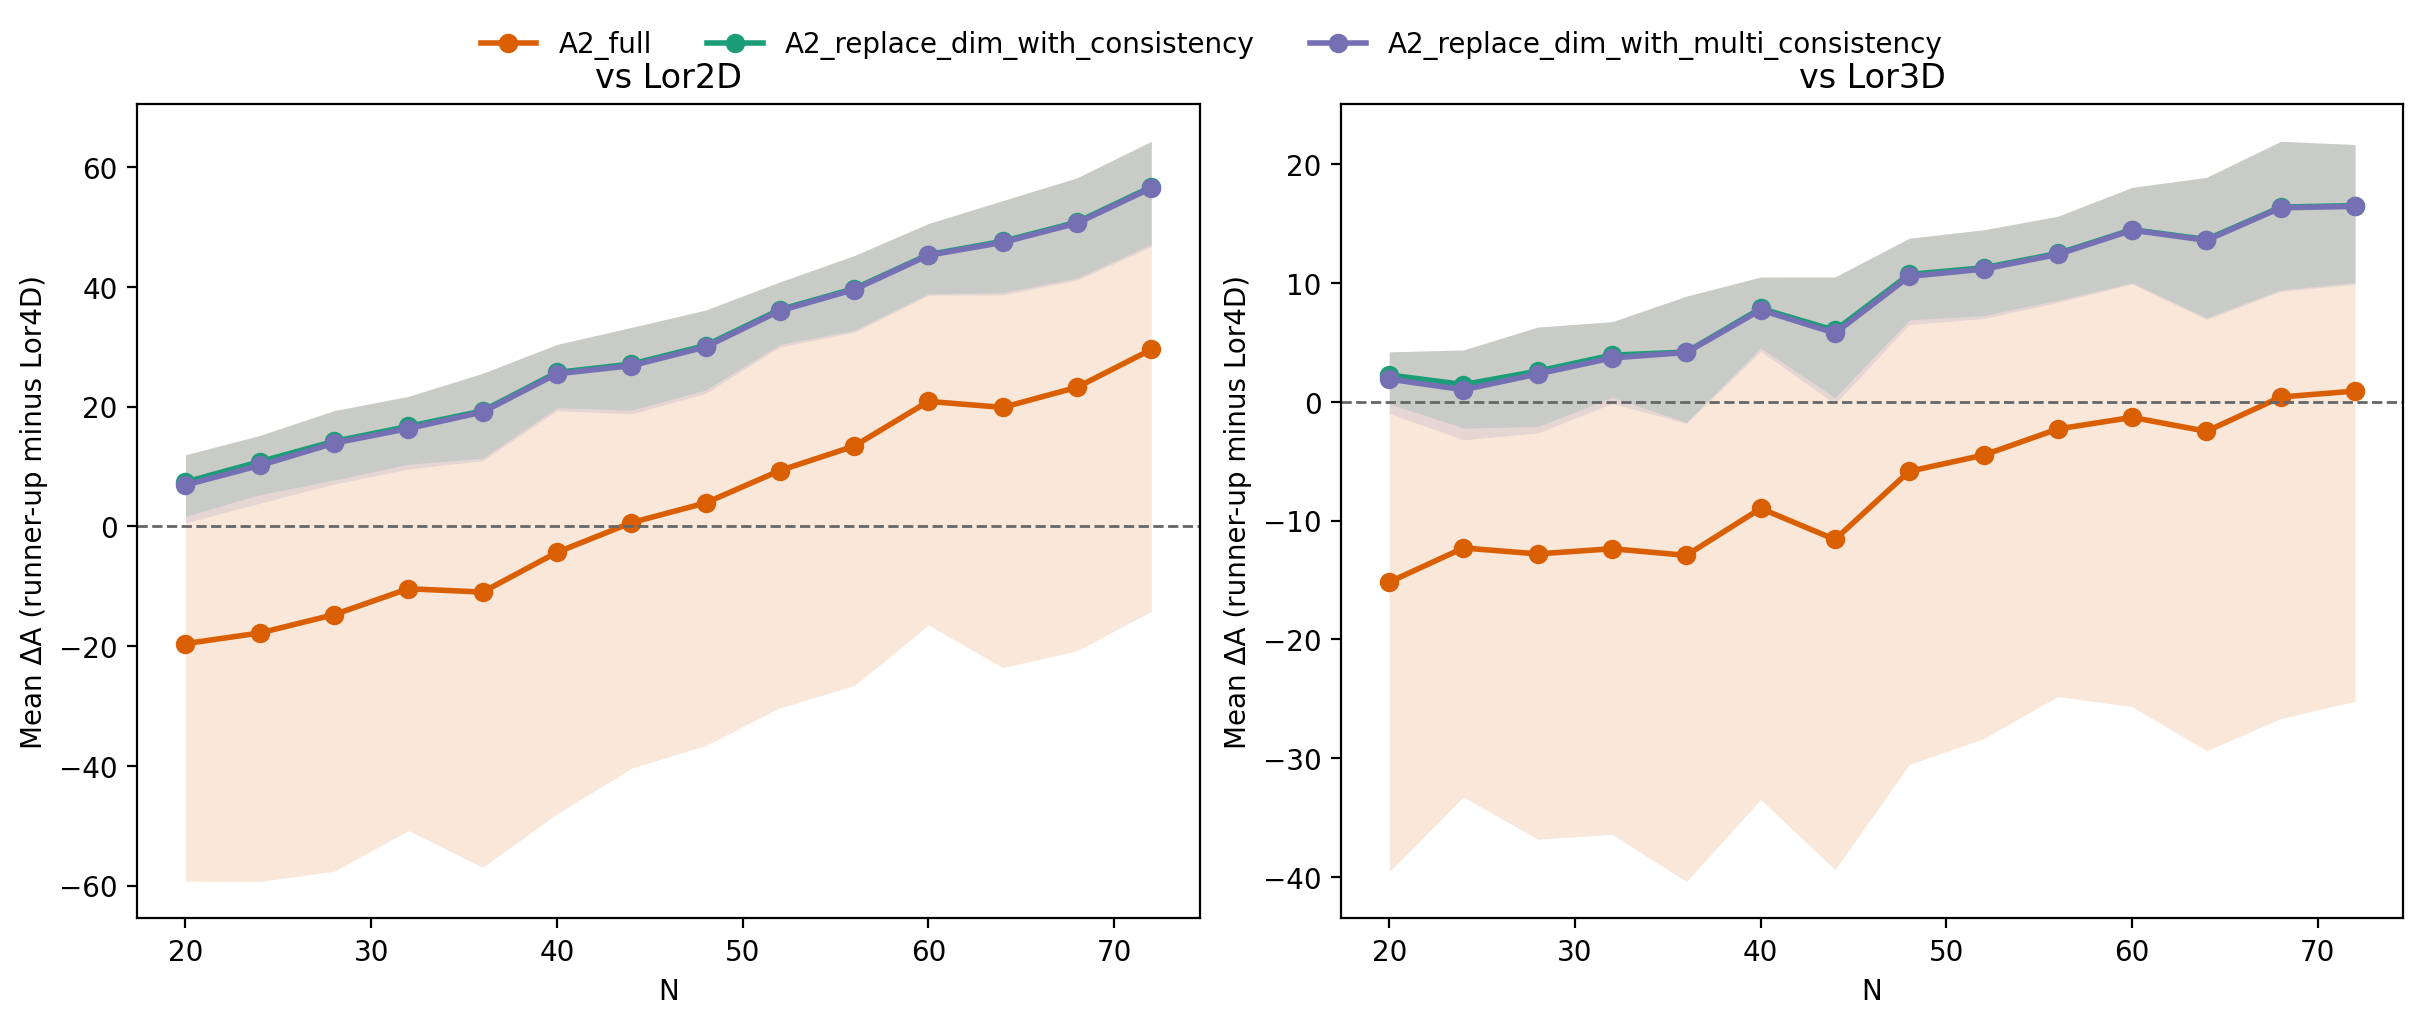
\includegraphics[width=0.9\columnwidth]{fig1_margin_of_victory.png}
    \caption{Margin of victory for \texttt{lor4d} over \texttt{lor2d} (blue)
    and \texttt{lor3d} (orange) under $A_2$ consistency, as a function of~$N$.
    Solid lines: mean margin across $\gamma$ values. Shaded regions: min--max
    range.}
    \label{fig:margin}
\end{figure}

The mean margin versus \texttt{lor2d} grows nearly linearly from $+7$ ($N = 20$)
to $+57$ ($N = 72$), and even the minimum margin is positive at every~$N$.
Against \texttt{lor3d}, the minimum margin becomes positive by $N = 44$ and
remains positive for all larger tested sizes.

% ════════════════════════════════════════════════════════════════════
\section{Robustness}
\label{sec:robustness}

\subsection{\texorpdfstring{Seed sensitivity at large $N$}{Seed sensitivity at large N}}
\label{sec:seed}

Experiments at $N = 64$, $68$, and $72$ with three independent generator seed
offsets (0, 50\,000, 100\,000) confirm robustness (Table~\ref{tab:seed}).

\begin{table}[h]
\centering
\caption{Seed sensitivity at $N = 64$, $68$, and $72$: winner counts out of 7
$\gamma$ values.}
\label{tab:seed}
\begin{tabular}{lcccc}
\toprule
\textbf{Variant} & $N$ & \textbf{Seed 0} & \textbf{Seed 50k} &
\textbf{Seed 100k} \\
\midrule
$A_2$ full & 64 & KR 4, L4d 3 & KR 3, L3d 1, L4d 3 & KR 2, L3d 2, L4d 3 \\
$A_2$ full & 68 & KR 4, L4d 3 & KR 4, L4d 3 & KR 4, L4d 3 \\
$A_2$ full & 72 & KR 4, L4d 3 & KR 4, L4d 3 & KR 4, L4d 3 \\
$A_2$ consistency & 64 & L4d 7/7 & L4d 7/7 & L4d 7/7 \\
$A_2$ consistency & 68 & L4d 7/7 & L4d 7/7 & L4d 7/7 \\
$A_2$ consistency & 72 & L4d 7/7 & L4d 7/7 & L4d 7/7 \\
\bottomrule
\end{tabular}
\end{table}

Under both consistency variants, \texttt{lor4d} achieves $100\%$ win rate
($63/63$ across all three $N$ values and all seeds). At $N = 68$ and $72$ the
KR--\texttt{lor4d} split under $A_2$ full is identical (4:3) at every
seed---a structural property of the action, not a sampling artifact. At
$N = 64$, the full action's winner is less stable, with \texttt{lor3d}
occasionally entering, consistent with the slight margin dip observed at that
scale.

\subsection{Consistency weight sensitivity}
\label{sec:wcon}

The calibrated weight $w_{\text{con}} = 0.6829$ was determined on the 7-family
ensemble. To verify that 4D dominance does not depend on this choice, we repeat
the $N = 20$--$36$ grid across eight weight values spanning nearly a factor of
four (Table~\ref{tab:wcon}).

\begin{table}[h]
\centering
\caption{Sensitivity of 4D dominance to consistency weight $w_{\text{con}}$
($N = 20$--$36$, 35 configurations each).}
\label{tab:wcon}
\begin{tabular}{ccccc}
\toprule
$w_{\text{con}}$ & \textbf{Lor4D} & \textbf{Lor3D} & \textbf{KR} &
\textbf{Lor2D} \\
\midrule
0.30 & 32 (91.4\%) & 3 & 0 & 0 \\
0.50 & 32 (91.4\%) & 3 & 0 & 0 \\
\textbf{0.6829} & \textbf{32 (91.4\%)} & \textbf{3} & \textbf{0} & \textbf{0} \\
0.80 & 33 (94.3\%) & 2 & 0 & 0 \\
1.00 & 34 (97.1\%) & 1 & 0 & 0 \\
1.20 & 34 (97.1\%) & 1 & 0 & 0 \\
\bottomrule
\end{tabular}
\end{table}

The 4D win rate is $\geq 91\%$ across the entire tested range
$w_{\text{con}} \in [0.3, 1.2]$, and \emph{increases} at larger weights.
Neither KR nor \texttt{lor2d} ever wins at any tested weight.

\subsection{Backbone weight sensitivity for \texorpdfstring{$\gamma_c$}{gamma\_c}}
\label{sec:wdim}

The calibrated dim-proxy weight $w_{\text{dim}} = 8$ was chosen via the
7-family grid. To verify that $\gamma_c$ responds smoothly, we repeat the
confirmatory exact scan at $N \in \{20, 28, 36, 44\}$ across three weight
values spanning a factor of 2.5 (Table~\ref{tab:wdim}).

\begin{table}[h]
\centering
\caption{Sensitivity of $\gamma_c$ to the dim-proxy weight $w_{\text{dim}}$
at four representative $N$.}
\label{tab:wdim}
\begin{tabular}{ccccc}
\toprule
$w_{\text{dim}}$ & $N = 20$ & $N = 28$ & $N = 36$ & $N = 44$ \\
\midrule
4  & 0.576 & 0.986 & 1.673 & 1.739 \\
\textbf{8 (baseline)} & \textbf{0.413} & \textbf{0.804} & \textbf{1.422} & \textbf{1.434} \\
10 & 0.362 & 0.736 & 1.322 & 1.319 \\
\bottomrule
\end{tabular}
\end{table}

Reducing $w_{\text{dim}}$ shifts $\gamma_c$ upward (the geometric penalty is
weaker, so a higher coupling is needed for Lor2D to overtake KR); increasing it
shifts $\gamma_c$ downward. The response is monotonic and continuous at every
tested~$N$, with no brittle jump or bifurcation, supporting the claim that the
bounded phase transition is a structural feature of the action rather than a
fine-tuned artifact.

\subsection{Out-of-grid validation}
\label{sec:oog}

To test generalization beyond the original parameter grid, we conduct an
independent validation on fresh $N$ and $\gamma$ values not used in any
previous experiment. We use $N \in \{22, 26, 30, 38, 42\}$ and
$\gamma \in \{0.1, 0.3, 0.5, 0.7, 0.9, 1.1, 1.5, 1.9\}$, with generator
seed offset $100\,000$ (Table~\ref{tab:oog}).

\begin{table}[h]
\centering
\caption{Out-of-grid validation: winner counts (40 configurations each).}
\label{tab:oog}
\begin{tabular}{lcccc}
\toprule
\textbf{Variant} & \textbf{Lor4D} & \textbf{KR} & \textbf{Lor2D} &
\textbf{Lor3D} \\
\midrule
$A_2$ full & 8 & 13 & 13 & 6 \\
$A_2$ consistency & 36 & 0 & 0 & 4 \\
$A_2$ multi-con. & 36 & 0 & 0 & 4 \\
\bottomrule
\end{tabular}
\end{table}

Under both consistency variants, \texttt{lor4d} wins $36/40$ ($90\%$) on the
fresh grid. In pairwise comparison, \texttt{lor4d} beats \texttt{lor2d} in
$40/40$ ($100\%$) under $A_2$ consistency. The 4 non-\texttt{lor4d} wins go to
\texttt{lor3d} at small-$N$, high-$\gamma$ configurations, consistent with the
in-grid pattern.

% ════════════════════════════════════════════════════════════════════
\section{Discussion}
\label{sec:discussion}

\subsection{Summary of evidence}

The numerical evidence supports two main findings:

\begin{enumerate}[nosep]
\item \textbf{Bounded phase transition.} Under $A_2$ with exact entropy, the
critical coupling $\gamma_c$ for \texttt{lor2d} to overtake \texttt{kr} exists
at all $N = 10$--$44$ and remains $O(1)$ (all values in $[0.146, 9.19]$; in
$[0.146, 0.995]$ for $N \geq 12$). This provides finite-size support for a
bounded geometric phase-transition threshold in poset ensembles.

\item \textbf{Dimensional selection.} Under the consistency replacement
($g_{\text{con}}$), \texttt{lor4d} is the dominant winner ($92/98$ in-grid,
$36/40$ out-of-grid, $63/63$ seed sensitivity, stable across
$w_{\text{con}} \in [0.3, 1.2]$) with a margin that grows with~$N$.
This indicates that dimensional consistency constraints, without
dimension-specific priors, can favor higher-dimensional Lorentzian
structures.
\end{enumerate}

The two results are connected: ablation identifies $g_{\text{dim}}$ as the
backbone term whose replacement requires care. The non-circular replacement
preserves the phase transition (Finding~1) while also changing the preferred
winner in the dimensional comparison (Finding~2). The mechanism depends on
dimensional \emph{consistency}, not dimensional \emph{identity}.

\subsection{Discriminative ceiling and Tier-2 families}
\label{sec:ceiling}

A candidate expansion experiment with 7 parameter-tunable random layered
families (Tier-2) revealed that these null-model posets can systematically
outperform \texttt{lor2d} under the current action for $N \geq 36$. This does
not invalidate the core claim (which is evaluated within Tier-1) but exposes a
discriminative ceiling: the action's observables are purely order-theoretic and
can be reverse-engineered by tuning layer parameters.

A structural discriminant separates the tiers cleanly: the normalized antichain
width $a_w / \sqrt{N}$ is near-constant at ${\sim}\,1.37$ for \texttt{lor2d}
(reflecting $\sqrt{N}$-scaling of the maximal antichain in Minkowski
sprinklings) versus $1.71\text{--}2.05$ for layered families,
$2.36\text{--}2.54$ for \texttt{lor3d}/\texttt{tp}, and
$3.09\text{--}3.14$ for \texttt{kr}/\texttt{lor4d}.
A Mann--Whitney $U$ test gives $p = 1.94 \times 10^{-28}$ for Lor2D vs.\ all
Tier-2 (720 samples). This ratio is already computable from existing observables
and provides a clean separation, though incorporating it into the action itself
is left for future work.

\subsection{Relation to prior work}

Work on causal set dynamics and on entropy barriers in causal set path sums is
substantial. Carlip~\cite{carlip2017} and Surya~\cite{surya2019} provide broad
reviews of dimensional reduction and causal set quantum gravity, including
discussions of entropy challenges and of finite-size effects. In a separate but
closely related direction, Loomis and Carlip~\cite{loomis2018} gave an analytic
argument that Einstein--Hilbert weighting in a Lorentzian causal set path
integral can suppress a large class of non-manifold-like structures (notably
two-level orders). Numerical studies of BD-based causal set quantum gravity in
low dimensions have explored phase-transition-like behavior and finite-size
scaling~\cite{surya2012,glaser2018}, with further developments in
dimensionally restricted settings~\cite{cunningham2020}. Our contribution is
different in focus: we compute an explicit finite-$N$ competition curve
$\gamma_c(N)$ using exact linear-extension measure factors in the confirmatory
window, and use decomposability to carry out controlled ablation and
replacement tests.

\textbf{Relation to the Benincasa--Dowker action.}
The BD action~\cite{benincasa2010,benincasa2011} is the standard discrete action
in CST, discretizing the Einstein--Hilbert action with a known continuum limit.
Our action $A_2$ differs in both form and purpose: it is a decomposable penalty
functional for ablation studies, not a discretization of a continuum action. The
advantage of decomposability is that systematic ablation can identify which
structural constraints drive geometric phase emergence---a diagnostic capability
that the BD action does not directly provide. Whether the BD action itself
produces a bounded $\gamma_c$ or exhibits dimensional preference under
consistency constraints remains open.

\subsection{Limitations}

\begin{enumerate}[nosep]
\item \textbf{Finite size.} Confirmatory exact data end at $N = 44$; the
bounded-$\gamma_c$ statement is a finite-$N$ observation, not a proof of
asymptotic boundedness.
\item \textbf{Finite family coverage.} 8 families (5 Tier-1, 3 Tier-2) do not
exhaust the space of possible poset types.
\item \textbf{Discriminative ceiling.} Tier-2 layered families expose the
action's order-theoretic limitations; more discriminative observables are needed.
\item \textbf{SIS estimation.} For $N > 32$ in non-\texttt{lor2d} families,
entropy is estimated rather than exact. Systematic biases at larger $N$ cannot
be fully excluded.
\item \textbf{Generator dependence.} The 4D generator's properties determine its
penalty values; different constructions might yield different results.
\item \textbf{``Higher dimension wins'' $\neq$ ``Why $3{+}1$?''} The result
shows that consistency constraints can select a dimension, not that
$3{+}1$ is uniquely selected. Additional constraints would be needed.
\item \textbf{$R_{2,\text{ref}}$ calibration.} The dimension estimator retains a
2D calibration constant ($R_{2,\text{ref}} = 0.5009$).
\end{enumerate}

\subsection{Outlook}

Three directions are natural: (i)~extending to 5D, 6D, and beyond to test
whether dominance continues or saturates at a preferred dimension;
(ii)~developing faster exact algorithms or hybrid methods to extend the
confirmatory window beyond $N = 44$; (iii)~incorporating the $a_w/\sqrt{N}$
discriminant or interval-geometric observables into the action to raise the
discriminative ceiling; (iv)~connecting the decomposable-action framework to BD
action dynamics to test whether the bounded phase transition and dimensional
selection survive under a physically grounded action.

% ════════════════════════════════════════════════════════════════════
\section{Conclusion}
\label{sec:conclusion}

We have studied two related questions in finite causal poset ensembles:

\begin{enumerate}[nosep]
\item A bounded geometric phase-transition threshold $\gamma_c$ under exact
entropy, with $\gamma_c \in [0.15, 1.00]$ for $N \geq 12$ across
$N = 10$--$44$.
\item Predominantly 4D Lorentzian outcomes under non-target-anchored consistency
constraints ($92/98$ in-grid, $36/40$ out-of-grid, $42/42$ seed-robust),
with margins that increase across the tested range.
\end{enumerate}

Both results trace to a common mechanism: ablation identifies a minimal
two-term backbone ($g_{\text{wh}} + g_{\text{dim}}$), and replacing the
target-anchored $g_{\text{dim}}$ with the consistency-based $g_{\text{con}}$
preserves the phase transition while changing the dimensional ordering. Within
the present finite ensembles, these results support the view that geometric
phase emergence and dimensional preference can arise from structural
self-consistency constraints in discrete causal-order models without requiring
dimension-specific priors.

% ════════════════════════════════════════════════════════════════════
\ifdoubleblind
\section*{Data Availability}

Code, configuration files, and output tables used in this study are archived
and will be provided to the editors and reviewers in anonymized form upon
request during peer review.

\else
\section*{Data Availability}

All code, configuration files, and output data are available at:
\href{https://github.com/unicome37/poset_phase}{GitHub repository}

Archived version:
\href{https://doi.org/10.5281/zenodo.18980657}{Zenodo archive (DOI: 10.5281/zenodo.18980657)}
\fi

% ── References ──────────────────────────────────────────────────────
\begin{thebibliography}{20}

\bibitem{bombelli1987}
L.~Bombelli, J.~Lee, D.~Meyer, and R.~D.~Sorkin,
``Space-time as a causal set,''
\textit{Phys.\ Rev.\ Lett.} \textbf{59}, 521--524 (1987).

\bibitem{sorkin2005}
R.~D.~Sorkin,
``Causal sets: Discrete gravity,''
in \textit{Lectures on Quantum Gravity}, ed.\ A.~Gomberoff and D.~Marolf
(Springer, 2005). arXiv:gr-qc/0309009.

\bibitem{kleitman1975}
D.~J.~Kleitman and B.~L.~Rothschild,
``Asymptotic enumeration of partial orders on a finite set,''
\textit{Trans.\ Amer.\ Math.\ Soc.} \textbf{205}, 205--220 (1975).

\bibitem{carlip2017}
S.~Carlip,
``Dimension and dimensional reduction in quantum gravity,''
\textit{Class.\ Quantum Grav.} \textbf{34}, 193001 (2017).
arXiv:1705.05417.

\bibitem{surya2019}
S.~Surya,
``The causal set approach to quantum gravity,''
\textit{Living Rev.\ Relativ.} \textbf{22}, 5 (2019).
arXiv:1903.11544.

\bibitem{loomis2018}
S.~P.~Loomis and S.~Carlip,
``Suppression of non-manifold-like sets in the causal set path integral,''
\textit{Class.\ Quantum Grav.} \textbf{35}, 024002 (2018).

\bibitem{dhar1978}
D.~Dhar,
``Entropy and phase transitions in partially ordered sets,''
\textit{J.\ Math.\ Phys.} \textbf{19}, 171 (1978).

\bibitem{promel2001}
H.~J.~Pr{\"o}mel, A.~Steger, and A.~Taraz,
``Phase transitions in the evolution of partial orders,''
\textit{J.\ Comb.\ Theory Ser.\ A} \textbf{94}, 230 (2001).

\bibitem{brightwell1991}
G.~Brightwell and P.~Winkler,
``Counting linear extensions,''
\textit{Order} \textbf{8}, 225--242 (1991).

\bibitem{mathur2021}
S.~Mathur, J.~S.~Singh, and S.~Surya,
``Entropy and the link action in causal set path sums,''
arXiv:2009.07232.

\bibitem{cunningham2020}
W.~J.~Cunningham and S.~Surya,
``Dimensionally restricted causal set quantum gravity: Examples in two and
three dimensions,''
\textit{Class.\ Quantum Grav.} \textbf{37}, 054002 (2020).
arXiv:1908.11647.

\bibitem{benincasa2010}
D.~M.~T.~Benincasa and F.~Dowker,
``The scalar curvature of a causal set,''
\textit{Phys.\ Rev.\ Lett.} \textbf{104}, 181301 (2010).
arXiv:0911.2725.

\bibitem{benincasa2011}
D.~M.~T.~Benincasa, F.~Dowker, and B.~Schmitzer,
``The random discrete action for two-dimensional spacetime,''
\textit{Class.\ Quantum Grav.} \textbf{28}, 105018 (2011).
arXiv:1011.5191.

\bibitem{rideout2000}
D.~P.~Rideout and R.~D.~Sorkin,
``A classical sequential growth dynamics for causal sets,''
\textit{Phys.\ Rev.\ D} \textbf{61}, 024002 (2000).
arXiv:gr-qc/9904062.

\bibitem{henson2006}
J.~Henson,
``The causal set approach to quantum gravity,''
in \textit{Approaches to Quantum Gravity}, ed.\ D.~Oriti
(Cambridge University Press, 2009). arXiv:gr-qc/0601121.

\bibitem{dowker2005}
F.~Dowker,
``Causal sets and the deep structure of spacetime,''
in \textit{100 Years of Relativity}, ed.\ A.~Ashtekar
(World Scientific, 2005). arXiv:gr-qc/0508109.

\bibitem{surya2012}
S.~Surya,
``Evidence for the continuum in 2D causal set quantum gravity,''
\textit{Class.\ Quantum Grav.} \textbf{29}, 132001 (2012).
arXiv:1110.6244.

\bibitem{glaser2018}
L.~Glaser,
``Finite size scaling in 2d causal set quantum gravity,''
\textit{Class.\ Quantum Grav.} \textbf{35}, 045002 (2018).
arXiv:1706.06432.

\bibitem{glaser2014}
L.~Glaser and S.~Surya,
``Towards a definition of locality in a manifoldlike causal set,''
\textit{Phys.\ Rev.\ D} \textbf{88}, 124026 (2013).
arXiv:1309.3403.

\end{thebibliography}

\end{document}
